\documentclass{beamer}
\usepackage{booktabs}
\usepackage{lmodern}
\usepackage{amsmath}
\usepackage{amssymb,amsmath}
\usepackage{ifxetex,ifluatex}
\usepackage{fixltx2e} % provides \textsubscript
\ifnum 0\ifxetex 1\fi\ifluatex 1\fi=0 % if pdftex
\usepackage[T1]{fontenc}
\usepackage[utf8]{inputenc}
\else % if luatex or xelatex
\ifxetex
\usepackage{mathspec}
\else
\usepackage{fontspec}
\fi
\defaultfontfeatures{Ligatures=TeX,Scale=MatchLowercase}
\fi
\providecommand{\tightlist}{%
\setlength{\itemsep}{0pt}\setlength{\parskip}{0pt}}
\setcounter{secnumdepth}{0}
\usepackage{xcolor}

% There are many different themes available for Beamer. A comprehensive
% list with examples is given here:
% http://deic.uab.es/~iblanes/beamer_gallery/index_by_theme.html
% You can uncomment the themes below if you would like to use a different
% one:
%\usetheme{AnnArbor}
%\usetheme{Antibes}
%\usetheme{Bergen}
%\usetheme{Berkeley}
%\usetheme{Berlin}
%\usetheme{Boadilla}
%\usetheme{boxes}
%\usetheme{CambridgeUS}
%\usetheme{Copenhagen}
%\usetheme{Darmstadt}
\usetheme{default}
%\usetheme{Frankfurt}
%\usetheme{Goettingen}
%\usetheme{Hannover}
%\usetheme{Ilmenau}
%\usetheme{JuanLesPins}
%\usetheme{Luebeck}
%\usetheme{Madrid}
%\usetheme{Malmoe}
%\usetheme{Marburg}
%\usetheme{Montpellier}
%\usetheme{PaloAlto}
%\usetheme{Pittsburgh}
%\usetheme{Rochester}
%\usetheme{Singapore}
%\usetheme{Szeged}
%\usetheme{Warsaw}

\title{Correlated bivariate Normal competing risks%  -- simulation findings in an ill-posed problem
}

% A subtitle is optional and this may be deleted
\subtitle{ -- simulation findings in an ill-posed problem}

\author{Malcolm~Hudson\inst{1,2} \and Valerie~Gares \inst{3} \and Maurizio~Manuguerra\inst{1} \and Val~Gebski\inst{2}}
% - Give the names in the same order as the appear in the paper.
% - Use the \inst{?} command only if the authors have different
%   affiliation.
%\institute[Macquarie University] % (optional, but mostly needed)
\institute
{
  \inst{1}%
  Macquarie University
  \and
  \inst{2}%
  NHMRC Clinical Trials Centre\\
  University of Sydney
  \and
  \inst{3}%
  INSA Rennes
}

\date{ISCB ASC 2018, Melbourne}

\subject{Competing Risks for bivariate Normal}
% This is only inserted into the PDF information catalog. Can be left
% out. 

% If you have a file called "university-logo-filename.xxx", where xxx
% is a graphic format that can be processed by latex or pdflatex,
% resp., then you can add a logo as follows:

\pgfdeclareimage[height=0.5cm]{MU-logo}{MQlogo.png}
\logo{\pgfuseimage{MU-logo}}

% Let's get started
\begin{document}

\begin{frame}
  \titlepage
\end{frame}

\begin{frame}{Outline}
  \tableofcontents
  % You might wish to add the option [pausesections]
\end{frame}

% Section and subsections will appear in the presentation overview
% and table of contents.
\section{Bivariate Normal Censored Linear Model}

\subsection{General approach}

\begin{frame}{Correlated competing risks model}
  \begin{itemize}
  \item
    Bivariate Normal Censored Linear Model (bnc lm)
    \begin{itemize}
    \item
      log-Time to \emph{first occurring} event
    \item
      Two events: $Y \sim \mbox{BVN}(\mu,\Sigma) $
    \item
      lm: $\mu = X B$
    \item
      \emph{bnc} lm for observed data: $y=\min (Y_1, Y_2, C)$;  $D=1,2,0$
    \end{itemize}
  \item
    Estimation
    \begin{itemize}
    \item ML solution 
    \item
      ML $\leftarrow$  MPL
    \item
      EM algorithm using imputed times to non-occurring event
    \end{itemize}
  \item 
    Imputation
    \begin{itemize}
    \item conditional moments
      \( E (Y_1| Y_1 > y, Y_2=y, \, D=2) \)
    \item
      \( E (Y_1| Y_1 > y, Y_2 > y, \, D=0) \)
    \item 
    \( E (Y_1^2| Y_1> y, Y_2=y,\, D=2) \) 
    \item
    \ldots \emph{etc}
    \end{itemize}
  \end{itemize}
\end{frame}



\subsection{EM algorithm for censored data}

\begin{frame}{BVN moment calculations for EM}
Simple example (for clarity)

\begin{itemize}
\item
  \emph{known} means of (log-)Normal latent vars, \emph{no censoring}
\item
  \(y=\min(Y_1,Y_2)\) with \(Y \sim \text{BVN}(0, \Sigma)\), \(\Sigma\)
  unknown
\item
  \(\Delta\) identifies which risk is observed (1 or 2)
\item
  two risk times are never \emph{both} observed
\item
  Goal: the ML estimator of \(\Sigma\) from an random sample of
  \(y, \Delta\)
\end{itemize}
\end{frame}


\section{Simulation Aim, Methods, Results}

\subsection{Simulation goals}

\begin{frame}{Simulation Goals and Outcomes}
\begin{itemize}
\item
  \alert{Aim:} parametric estimation of \alert{first-event data} from correlated
  BVN competing risks

  \begin{itemize}
  \tightlist
  \item
    Sampling distribution (\alert{bias, variance}) of MPL estimation of
    BVN parameters in one- and two- sample datasets  first-event times
  \item
    Sampling distribution of mean difference estimated between Treated
    and Control subjects
  \end{itemize}

\item Simulation outcomes
  \begin{itemize}
  \tightlist
  \item Bias and Variance in ML estimation of parameters (esp. \( \rho \) ) in BVN\( (\mu,\Sigma) \)
  \item Convergence status, number of iterations
  \item varying: sample size, tolerance (cvg)
  \end{itemize}
\end{itemize}
\end{frame}


\hypertarget{results}{%
\section{Simulations}\label{simulations}}

\begin{frame}[fragile]{Methods}
\protect\hypertarget{methods}{}

\begin{itemize}
\tightlist
\item
  One- and two-sample simulations, BVN and \emph{non-}Normal copula
  (with Normal margins)

  \begin{itemize}
  \tightlist
  \item
    Parameters varying

    \begin{enumerate}
    [i.]
    \tightlist
    \item
      Sample size (100, {\color{red}{400}}, 1000)  {\color{red}{why not 500}}
    \item
      Mean difference event-of-interest to competing-event (0, 0.5, 1)
    \item
      Event probability (complement \emph{censoring fraction}) $\to$ prob event-of-interest occurs before \texttt{eof}
        \begin{itemize}
        \tightlist
        \item[~~-]
          Surviving fractions (1, 0.8, 0.6)
        \item[~~-]
          Competing event censoring \emph{not} included
        \end{itemize}
    \item
      \alert{Correlation} \(\rho \in (-0.5,-0.25, 0, 0.25, 0.5)\)
    \item
      \alert{Treatment benefit} (mean difference between \emph{Treated
      and Controls, 2 sample only})
    \end{enumerate} % params varying
  \end{itemize}

\item
  Parallel simulation computation
  \begin{itemize}
  \tightlist
  \item
    \textbf{simsalapar} R package Hofert and Mächler (2016)
  \end{itemize}

\item
  Fixed-point accelerated EM iterations Bobb and Varadhan (2014)
\item
  estimation conducted in our R package \textbf{bnc}
\end{itemize}

\end{frame}

\setbeamertemplate{itemize subitem}[triangle] % Pour le deuxième niveau
\setbeamertemplate{itemize subsubitem}[square] % Pour le troisième niveau
%\setbeamerfont*{itemize item}{size=\scriptsize}
\setbeamercolor{itemize item}{}
\setbeamercolor{itemize subitem}{fg=orange}
\setbeamercolor{itemize subsubitem}{fg=orange}

\setbeamerfont{headline}{size=\Large}\section{Results:}

%%

\section{{1-sample} estimation of correlation}
\protect\hypertarget{estimation-of-rho-one-sample}{}


\begin{frame}{squareEM iterations (n=1000)}

\begin{table}[htbp]
  \centering\scriptsize
  \begin{tabular}{*{2}{l}*{3}{r}}
    \toprule
    cs & \( \rho \) \textbar\ beta2 & \multicolumn{1}{c}{0} & \multicolumn{1}{c}{0.5} & \multicolumn{1}{c}{1} \\
    \midrule
    1 & -0.5 & 36 & 95 & 93 \\
    & -0.25 & 83 & 107 & 154 \\
    & 0 & 107 & 142 & {\color{red}250} \\
    & 0.25 & 90 & 127 & {\color{red}250} \\
    & 0.5 & 112 & 227 & {\color{red}250} \\ \addlinespace[3pt]
    0.8 & -0.5 & 36 & 90 & 116 \\
    & -0.25 & 88 & 108 & 243 \\
    & 0 & 119 & 163 & {\color{red}250} \\
    & 0.25 & 146 & 219 & {\color{red}250} \\
    & 0.5 & 141 & 248 & {\color{red}250} \\ \addlinespace[3pt]
    0.6 & -0.5 & 78 & 105 & {\color{red}250} \\
    & -0.25 & 117 & {\color{red}250} & 235 \\
    & 0 & 134 & 212 & {\color{red}250} \\
    & 0.25 & 159 & 240 & {\color{red}250} \\
    & 0.5 & 184 & {\color{red}250} & {\color{red}250} \\
    \bottomrule
  \end{tabular}
  \caption*{max number iterations to converge, nsim=100}
  \label{tab:ft1b}
\end{table}
\end{frame}




\begin{frame}{Correlation (n=100)}

\begin{center}
  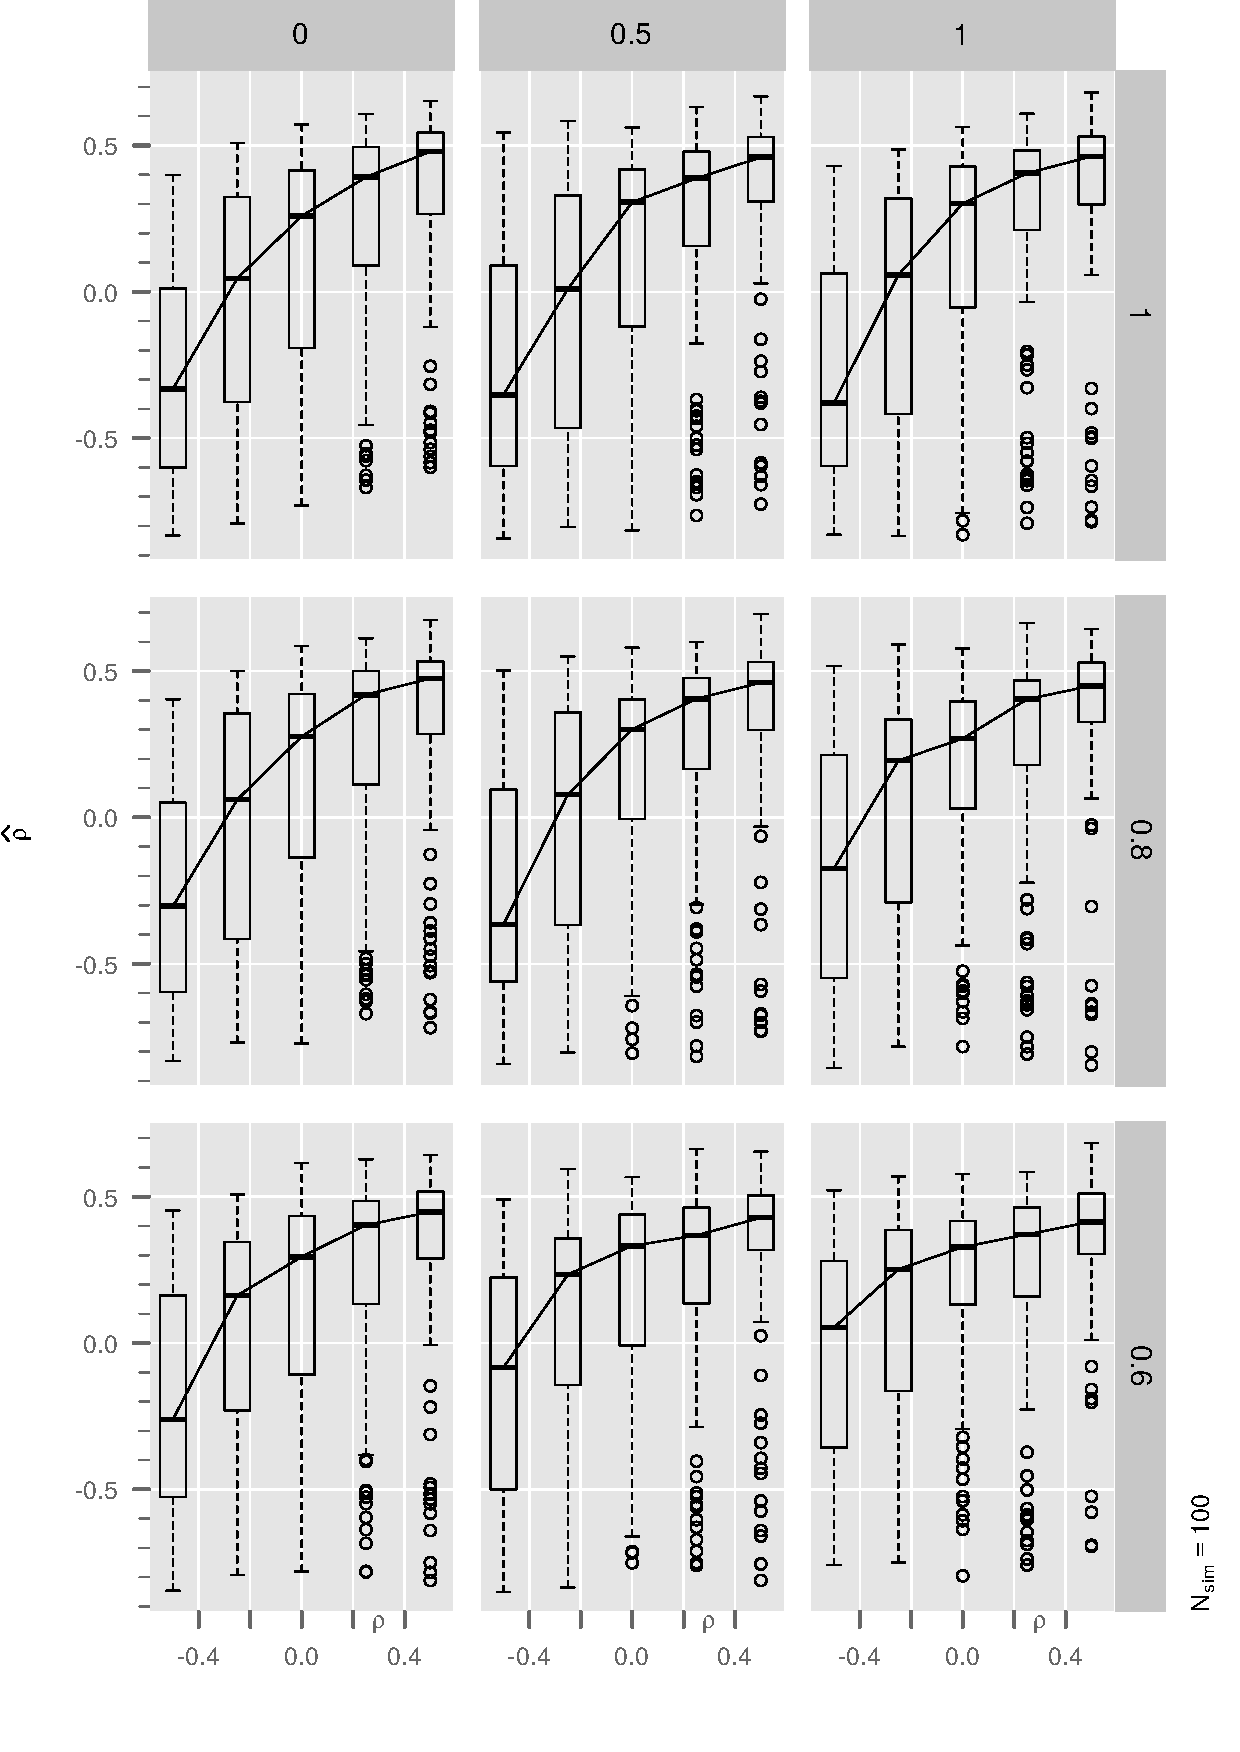
\includegraphics[trim= 0cm 0cm 0cm 11.75cm, clip, scale=0.475]{Figure1/tbl1_n100_rho_mayplot.pdf}
\end{center}

\end{frame}

\begin{frame}{Correlation, n=500 (Density plot)}

\begin{center}
  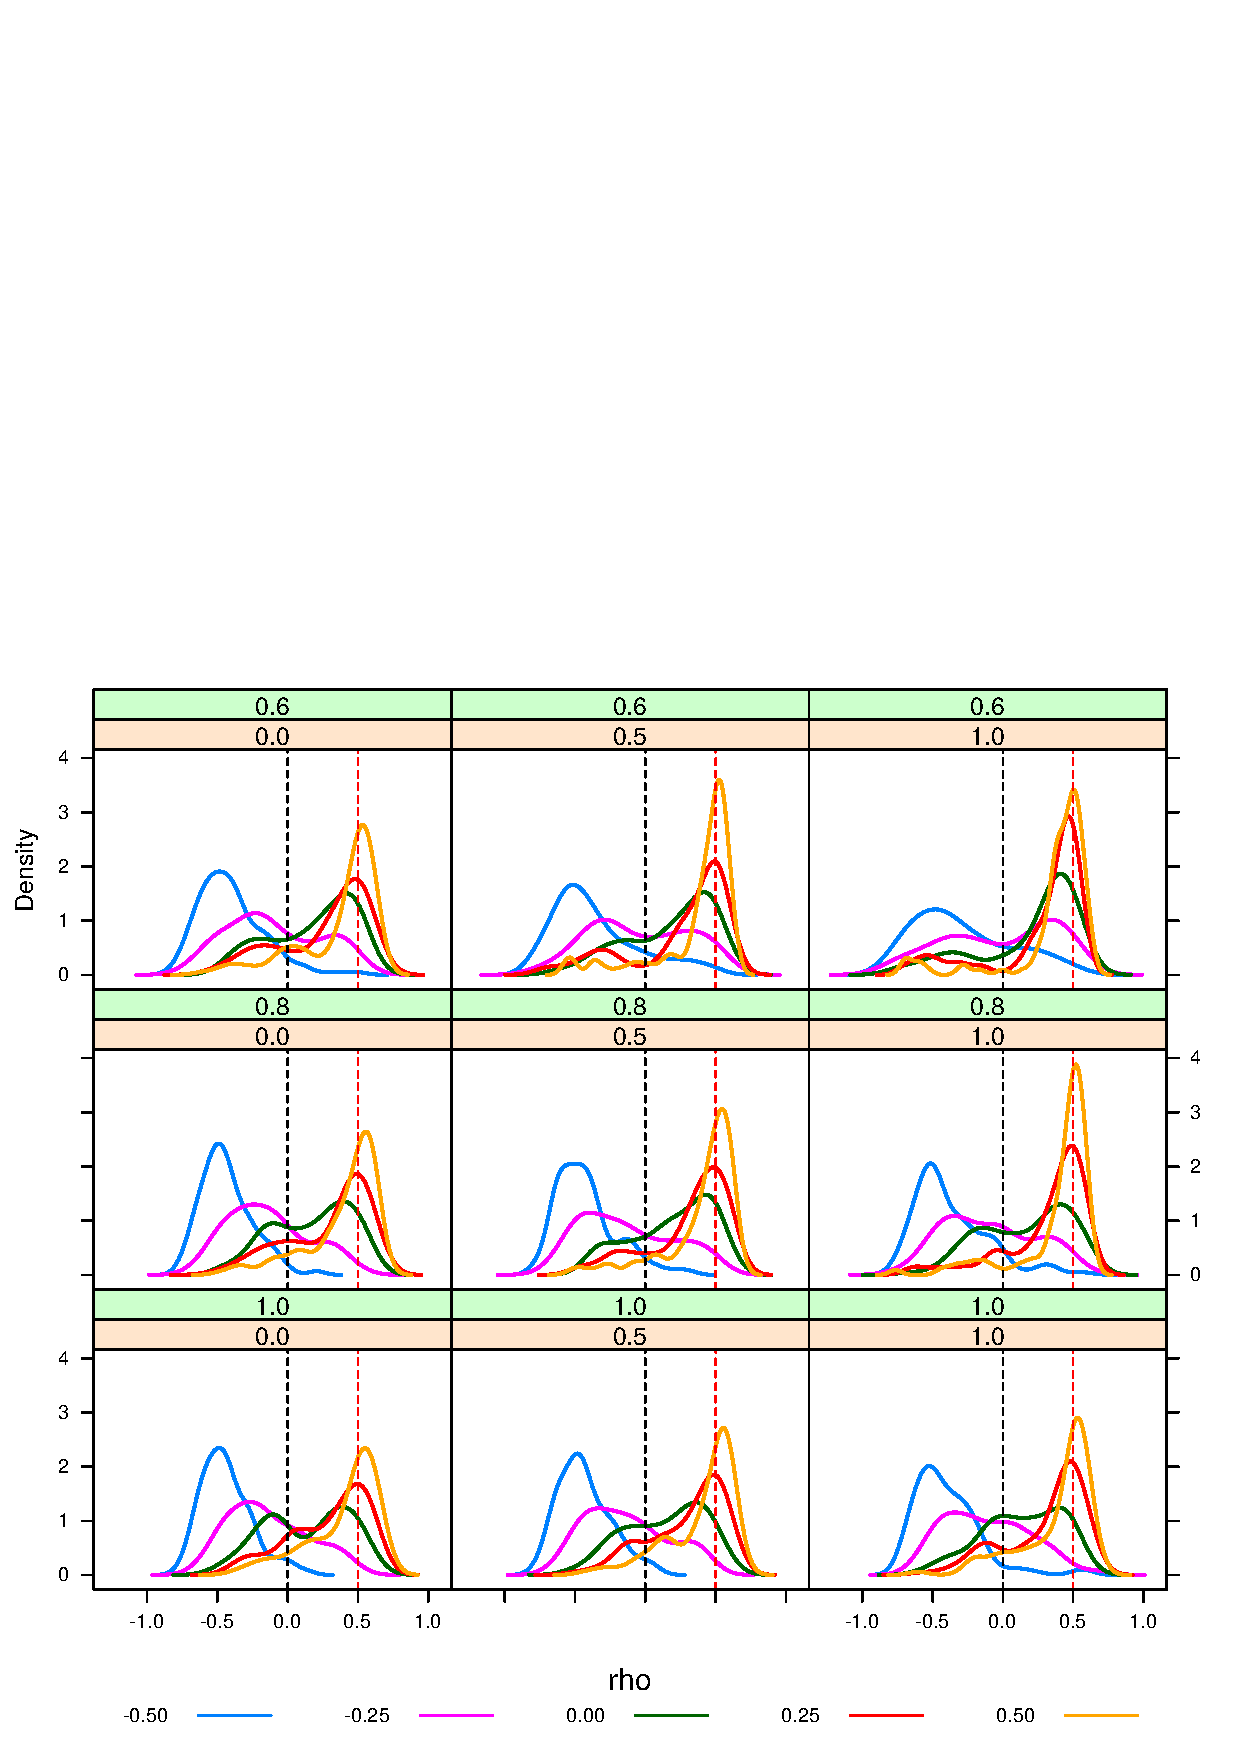
\includegraphics[trim= 0cm 0cm 0cm 11.75cm, clip, scale=0.47]{Figure1/tbl1densityPlot_n500.pdf} % width=1.00\textwidth, clip,, [scale=0.67]
\end{center}

\end{frame}

% ==============================================================================================
\section{{2-sample} estimation of treatment benefit}
\protect\hypertarget{two-samples}{}

\begin{frame}{Treatment Benefit $\hat{\Delta}=\hat{\beta}_{21}$ (n=1000)} % 3b: n=1000
\begin{table}[htbp]
  \centering\scriptsize
  \begin{tabular}{*{2}{l}*{4}{r}}
    \toprule
     & beta12 & \multicolumn{2}{c}{0} & \multicolumn{2}{c}{1} \\
    \cmidrule(lr){3-4} \cmidrule(lr){5-6}
    cs & \( \rho \) \textbar\ deltaTreat & \multicolumn{1}{c}{0} & \multicolumn{1}{c}{0.5} & \multicolumn{1}{c}{0} & \multicolumn{1}{c}{0.5} \\
    \midrule
    1 & -0.5 & -0.00 & 0.50 & 0.00 & 0.51 \\
    & -0.25 & -0.00 & 0.48 & -0.01 & 0.50 \\
    & 0 & 0.00 & 0.46 & 0.00 & 0.50 \\
    & 0.25 & -0.01 & 0.49 & 0.00 & 0.49 \\
    & 0.5 & -0.00 & 0.52 & -0.00 & 0.49 \\ \addlinespace[3pt]
    0.8 & -0.5 & -0.00 & 0.50 & 0.00 & 0.50 \\
    & -0.25 & -0.00 & 0.48 & 0.01 & 0.49 \\
    & 0 & 0.01 & 0.49 & 0.00 & 0.49 \\
    & 0.25 & -0.00 & 0.48 & -0.01 & 0.48 \\
    & 0.5 & -0.01 & 0.51 & 0.01 & 0.51 \\ \addlinespace[3pt]
    0.6 & -0.5 & 0.02 & 0.49 & -0.01 & 0.48 \\
    & -0.25 & -0.02 & 0.52 & -0.00 & 0.48 \\
    & 0 & -0.01 & 0.49 & 0.01 & 0.48 \\
    & 0.25 & 0.02 & 0.49 & 0.01 & 0.50 \\
    & 0.5 & 0.00 & 0.51 & -0.01 & 0.51 \\
    \bottomrule
    \multicolumn{5}{l}{\footnotesize{medians of 100 replicates}} % \multicolumn{4}{l}{\textsuperscript{*}\footnotesize{The footnote}}
  \end{tabular}
%  \caption{b21 TreatDiff estimate: Table 3b, n=1000}
  \label{tab:ft21}
\end{table}

\end{frame}


%\begin{frame}{2-sample: Treatment Benefit, n=1000 (estimates)} % sf x beta12

%\begin{center}
%  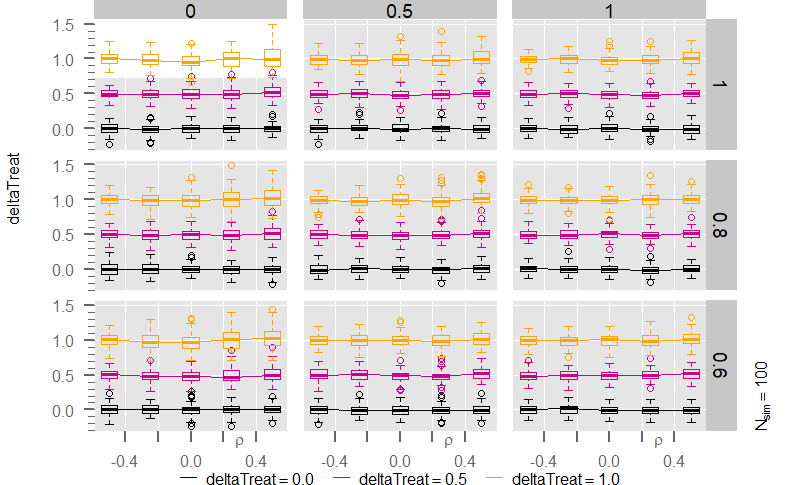
\includegraphics[width=1.00\textwidth]{Figure3/mayplot3-deltaTreat-n1000.png}
%\end{center}

%\end{frame}

%{Treatment Benefit, n=1000, sf=0.6 (density plots)}
%  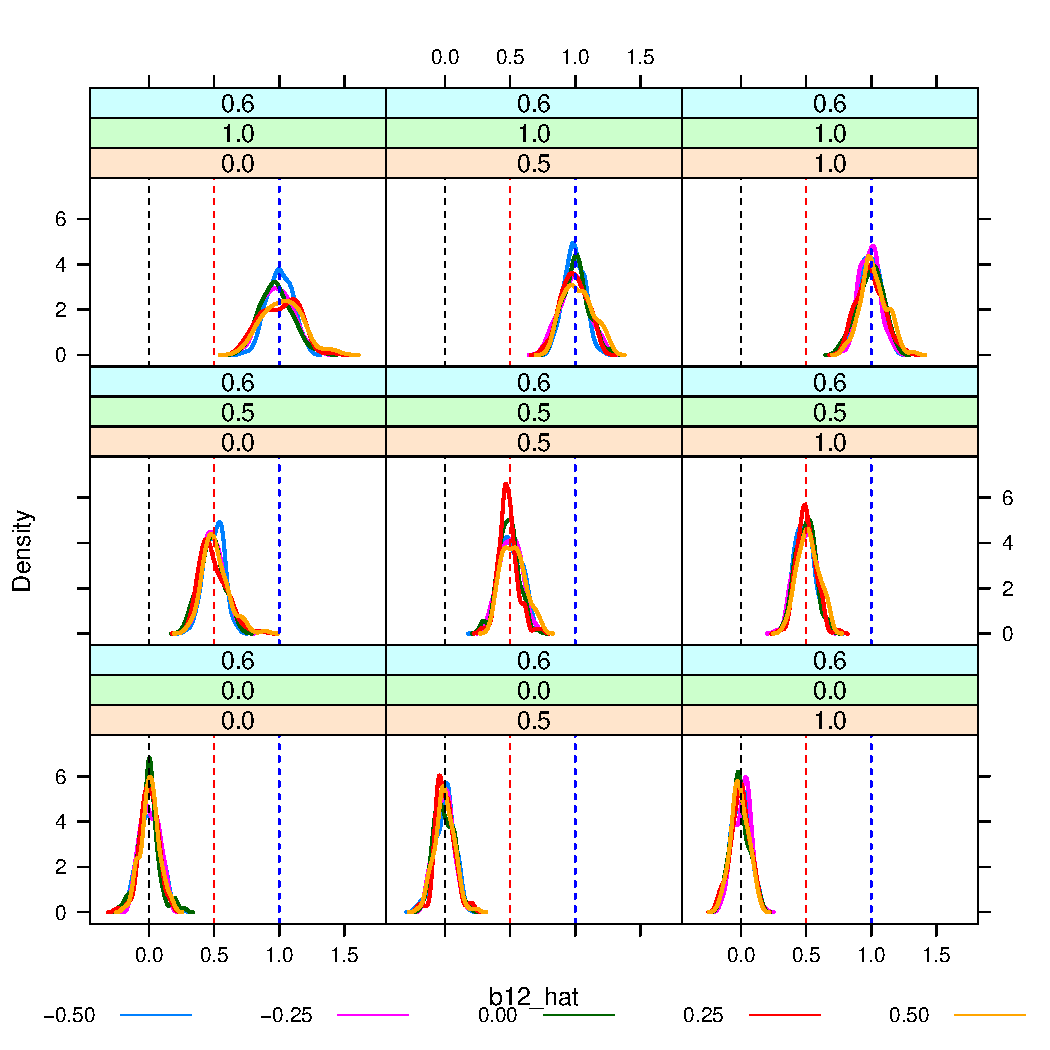
\includegraphics[scale=0.45]{Figure3/tbl3DensityPlots_n1000_003.pdf} % sf=0.6

\begin{frame}{Treatment Benefit, n=100 (estimates)} % sf x beta12

\begin{center}
  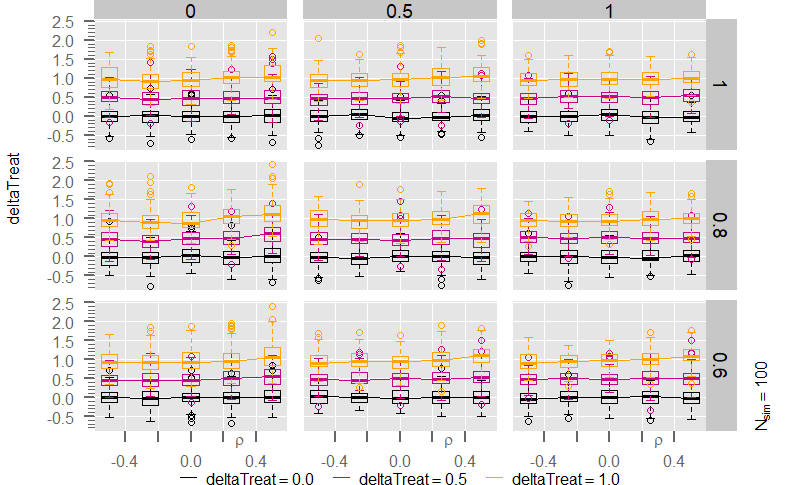
\includegraphics[width=1.00\textwidth]{Figure3/mayplot3-deltaTreat-n100.png}
\end{center}

\end{frame}

%  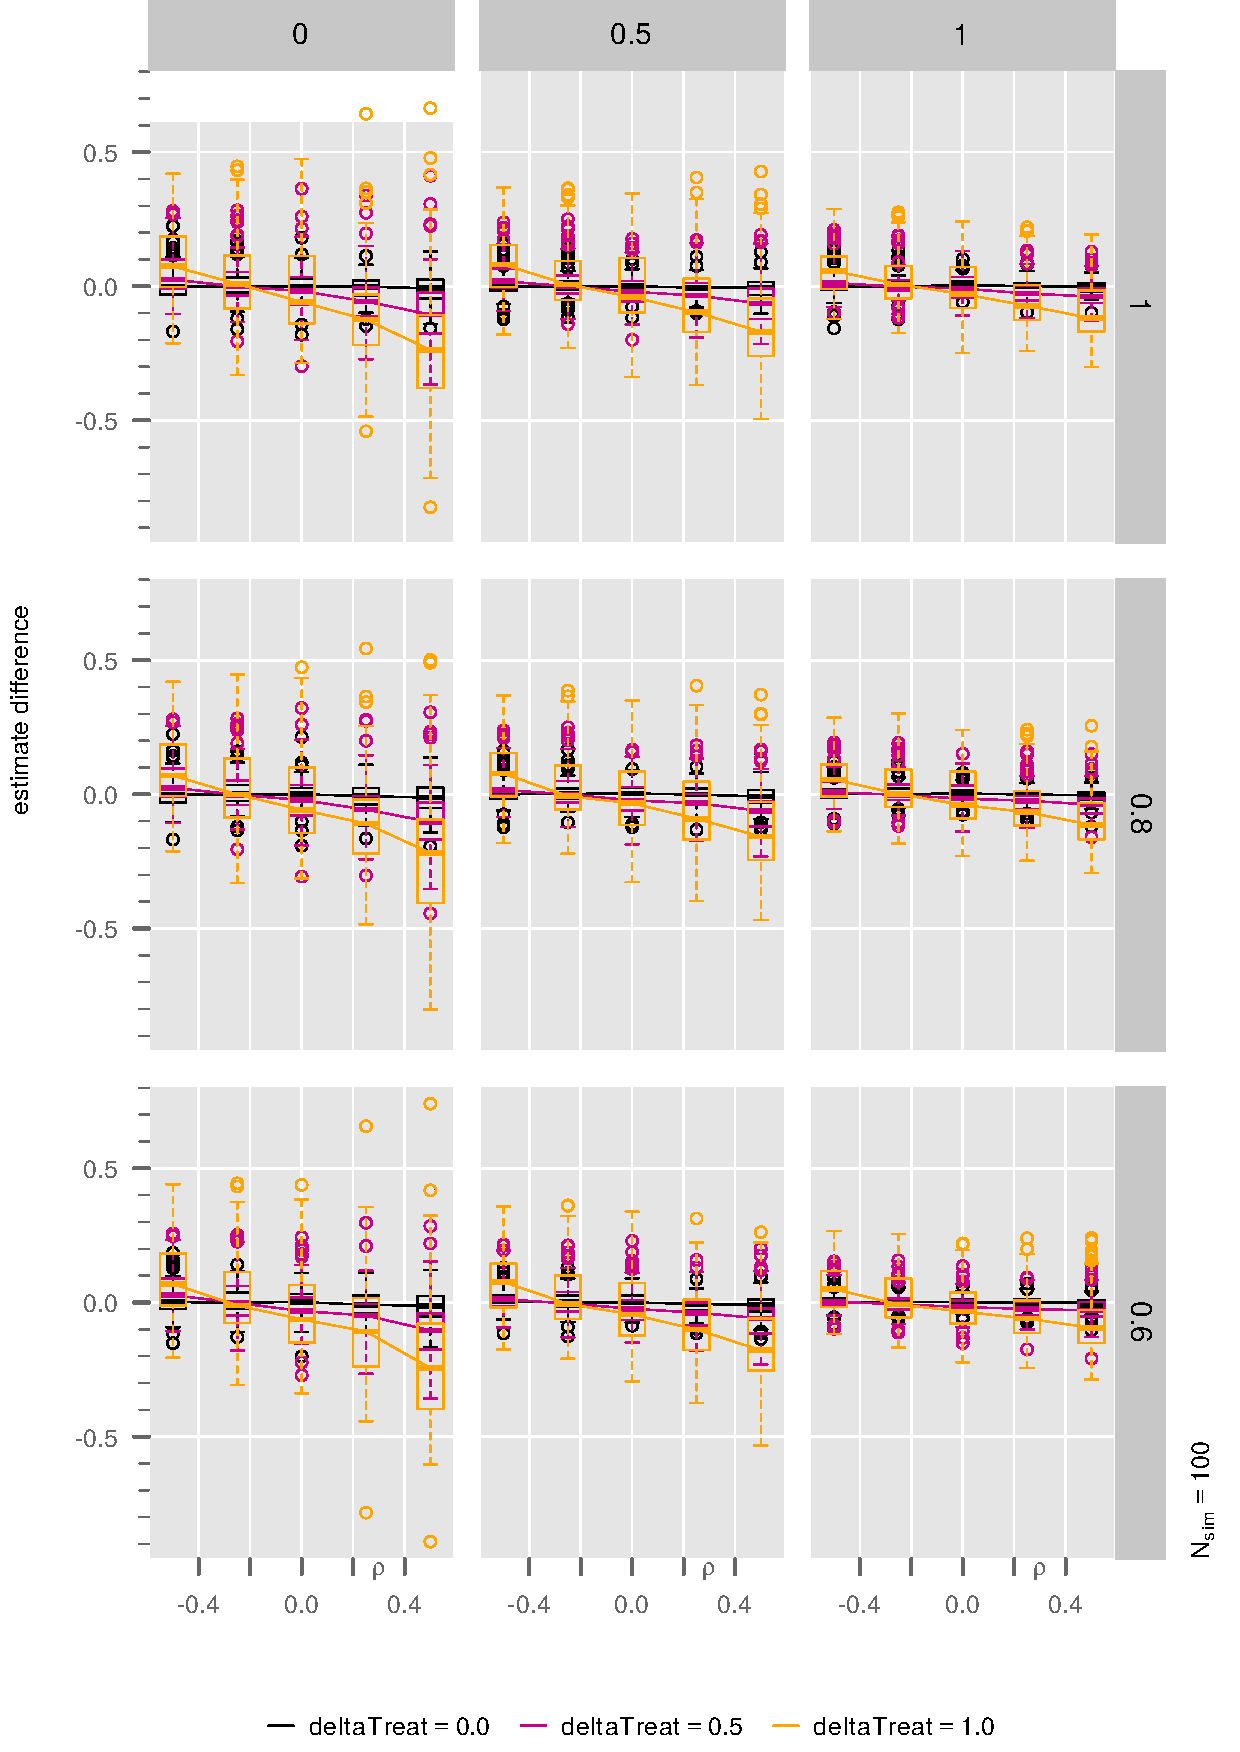
\includegraphics[width=0.95\textwidth]{Figure3/estimateDifferences2v12.pdf}


%\begin{frame}{2-sample: Treatment difference: BNC estimate  vs survreg coef ($\rho=0$)}

%\begin{center}
%  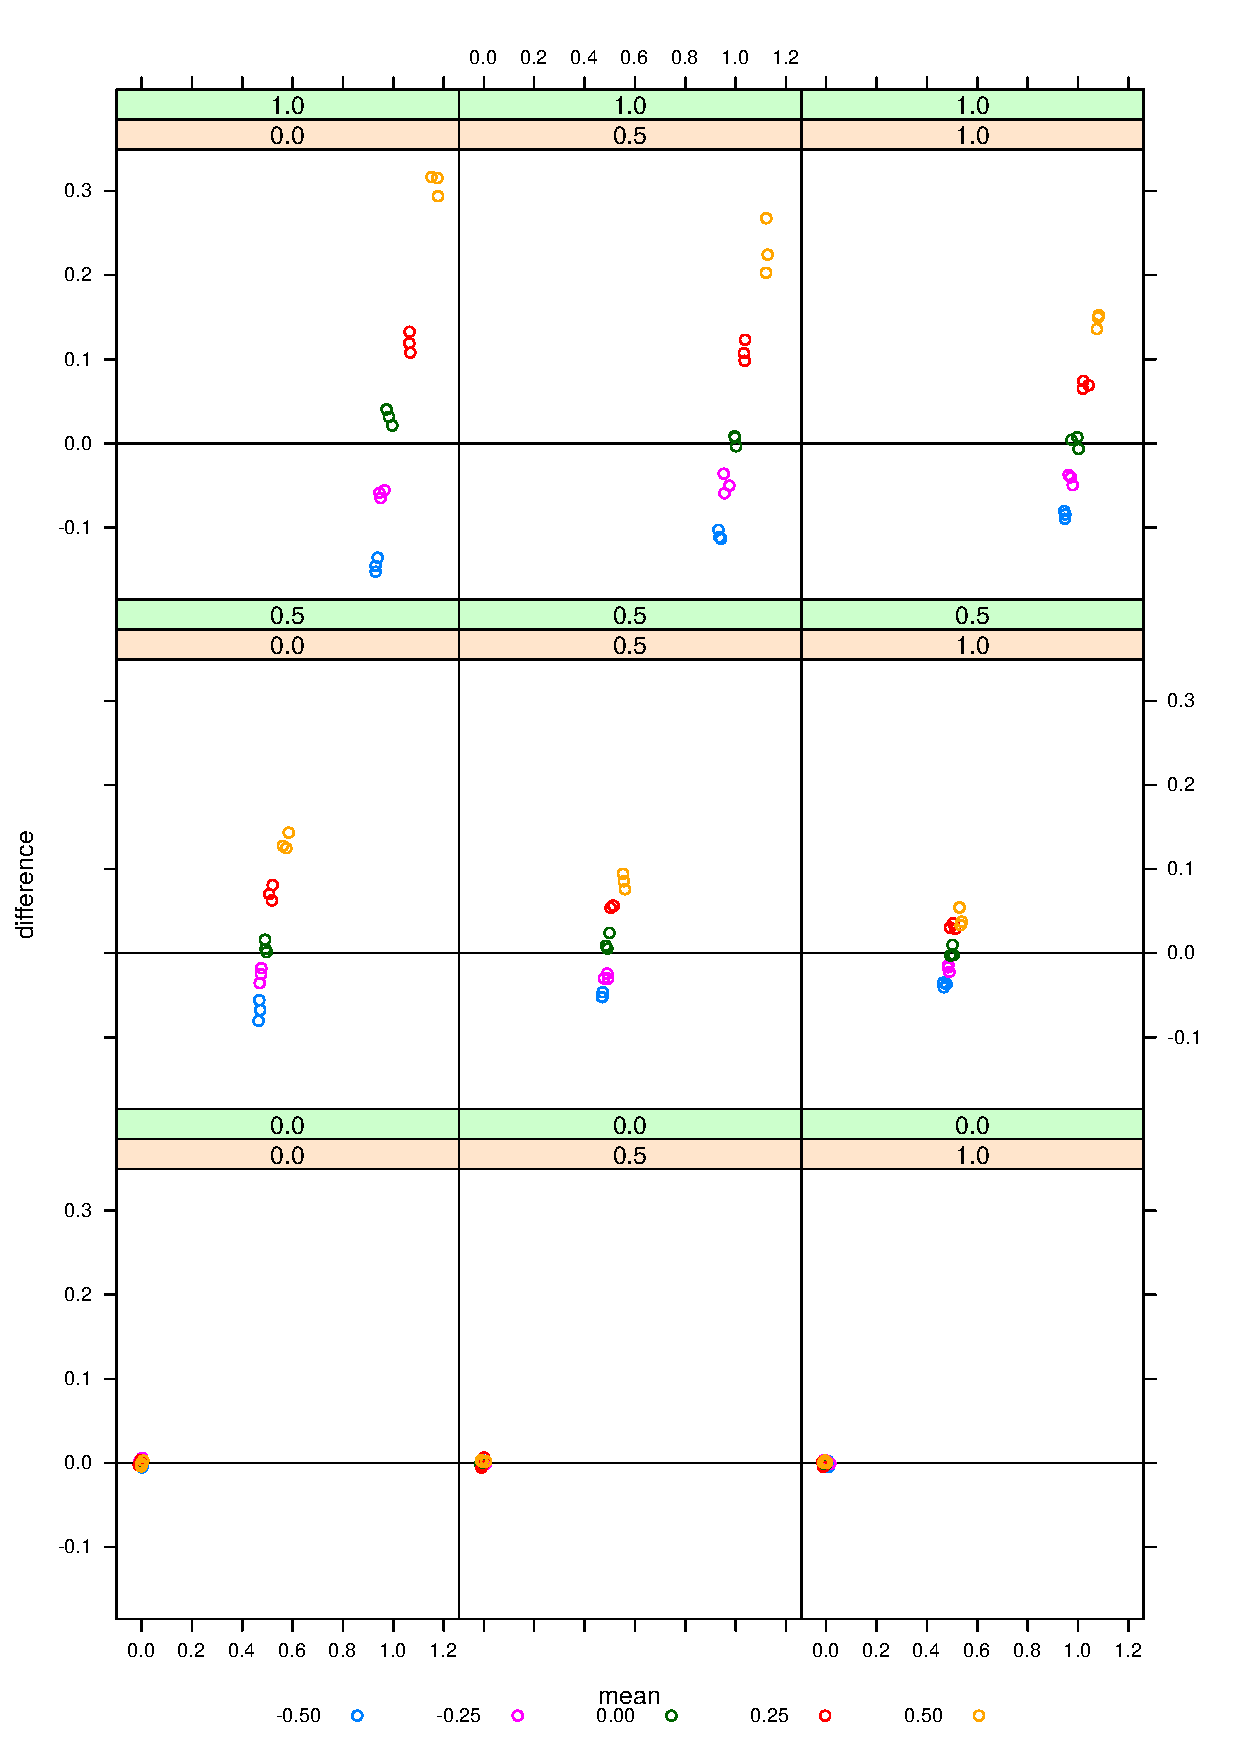
\includegraphics[height=0.95\textheight,width=0.95\textwidth]{%
%  Figure3/estimateDifferences2vs12v2.pdf%
%  }
%\end{center}

%\end{frame}


\begin{frame}{Treatment Benefit, n=1000, sf=0.6 (density plots)}

\begin{center}
  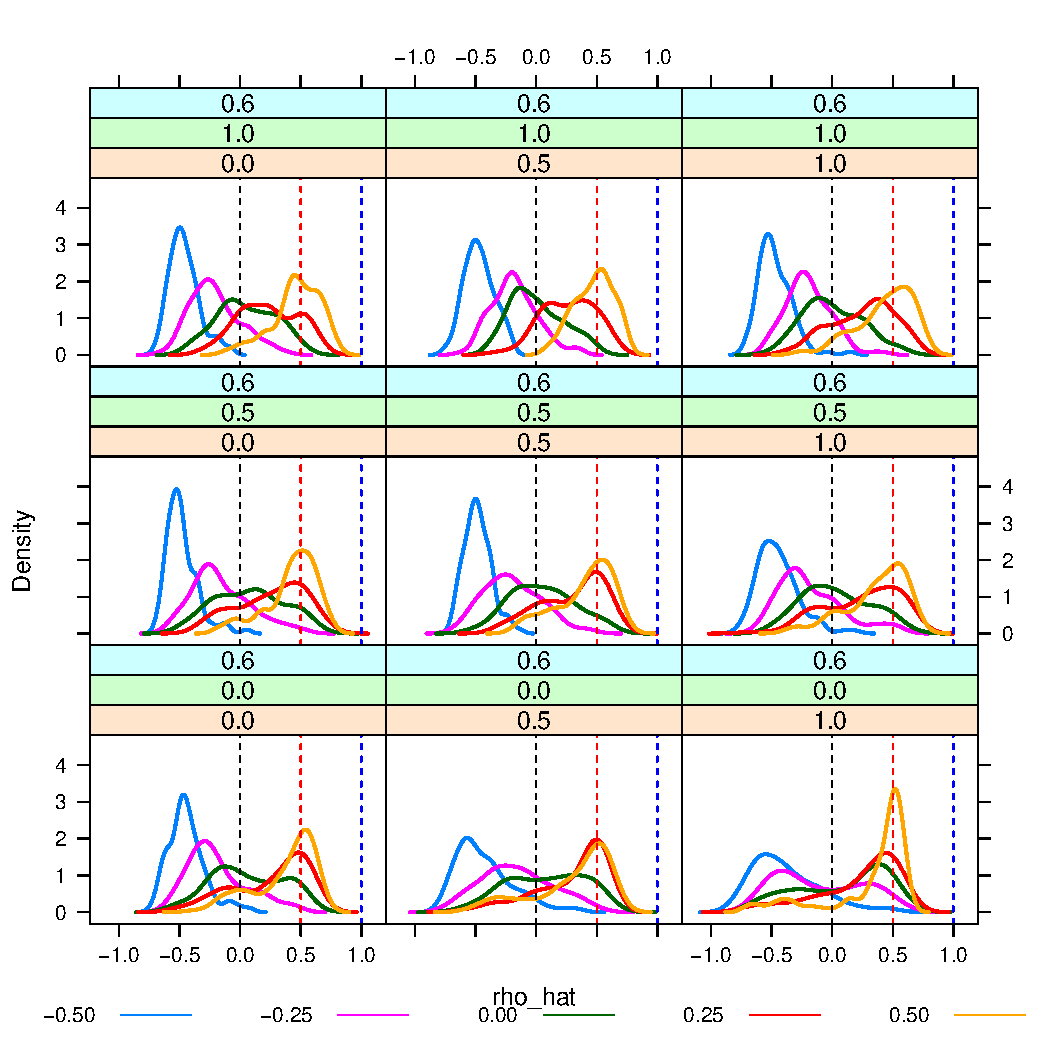
\includegraphics[scale=0.45]{Figure3/tbl3DensityPlots_rho_n1000_003.pdf} % sf=0.6
\end{center}

\end{frame}




\section{Consequences}

\subsection{Fixed correlation, a la GEE}

\begin{frame}{Fixed correlation }
\begin{block}{$\rho=0$}
Since estimating $\rho$ is unstable, perhaps better to fix it (a priori to 0). 
\end{block}

\end{frame}

\begin{frame}{}
    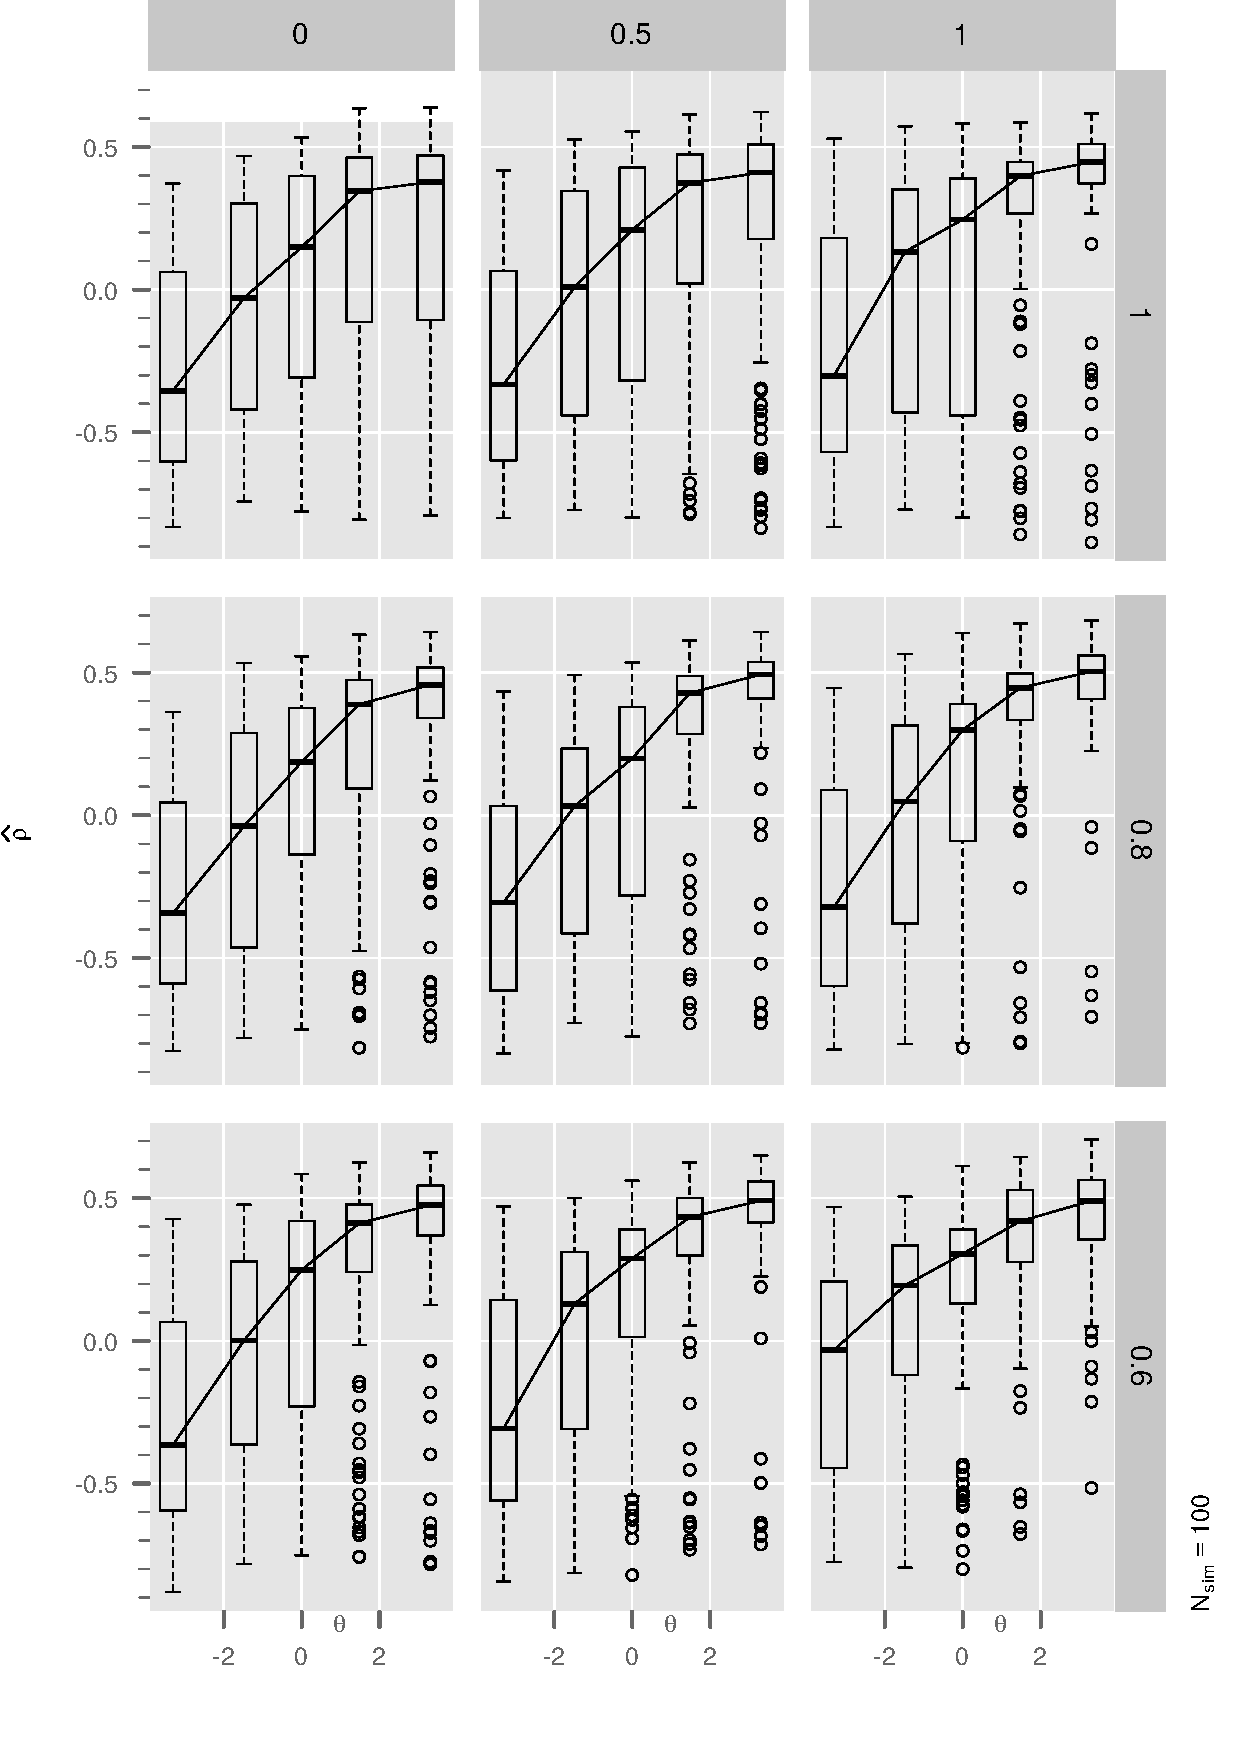
\includegraphics[width=1.00\textwidth]{Figure2/boxplotArray2.pdf} % [width=150pt]
\end{frame}

\subsection{Robustness to non-Normality}

\begin{frame}{}
\begin{exampleblock}{Frank's copula}
\begin{itemize}
    \item we set standard Normal marginals
    \item association parameter, Franks $\theta$
\end{itemize}
\end{exampleblock}
\end{frame}
% Placing a * after \section means it will not show in the
% outline or table of contents.
\section*{Summary}

\begin{frame}[fragile]{So you want to fit BVN to two competing risks?}
\protect\hypertarget{so-you-want-to-fit-bvn-to-two-competing-risks}{}
\setbeamercovered{transparent}
\begin{itemize}
\tightlist
\item<1->
  optimize to maximize Likelihood (\emph{routine})
  \item<2-> EM algorithm (\emph{safety first}) 
  \item<3-> mildly
penalize Likelihood, adjust EM alg for MPL
  \item<4-> accelerate EM (Aitken via squareEM)
  \item<5-> change start-point: initial small number of
EM iterations 
  \item<6-> R-package \textbf{bnc}
\end{itemize}

\alert{\emph{What could possibly go wrong?}}
\begin{itemize}
\item<1> singular Hessian, failure to remain in $-1 < \rho < 1$ 
\item<2>
  \begin{enumerate}
  \item[i.] be prepared to wait (forever) for convergence;
  \item[ii.] convergence failure possible when $\hat{\rho} = +1$ or $-1$
  \end{enumerate}
\item<3> still very slow, but sure, convergence
\item<4> very fast, but can fail to converge
\end{itemize}
\end{frame}

\begin{frame}{Summary}
  \begin{itemize}
  \item
    The \alert{first main message} of your talk in one or two lines.
  \item
    The \alert{second main message} of your talk in one or two lines.
  \item
    Perhaps a \alert{third message}, but not more than that.
  \end{itemize}
  
  \begin{itemize}
  \item
    Outlook
    \begin{itemize}
    \item
      Something you haven't solved.
    \item
      Something else you haven't solved.
    \end{itemize}
  \end{itemize}
\end{frame}






% \hypertarget{references}{%

\section{References}\label{references}

\begin{frame}[allowframebreaks]{References}
\label{References}

Aitkin, M. 1981. ``A Note on the Regression Analysis of Censored Data.''
\emph{Technometrics} 23 (2). American Statistical Association; American
Society for Quality: 161--63. \url{http://www.jstor.org/stable/1268032}.

%\leavevmode\hypertarget{ref-Rpackage-turboEM}{}%
Bobb, Jennifer F., and Ravi Varadhan. 2014. \emph{TurboEM: A Suite of
Convergence Acceleration Schemes for EM, MM and Other Fixed-Point
Algorithms}. \url{https://CRAN.R-project.org/package=turboEM}.

%\leavevmode\hypertarget{ref-Crowder1991}{}%
Crowder, M. 1991. ``On the Identifiability Crisis in Competing Risks
Analysis.'' \emph{Scandinavian Journal of Statistics}
18 (3): 223--33. \url{https://doi.org/10.2307/4616205}.

%\leavevmode\hypertarget{ref-Rpackage-simsalapar}{}%
Hofert, Marius, and Martin Mächler. 2016. ``Parallel and Other
Simulations in R Made Easy: An End-to-End Study.'' \emph{Journal of
Statistical Software} 69 (4): 1--44.
\url{https://doi.org/10.18637/jss.v069.i04}.

%\leavevmode\hypertarget{ref-JeongFine2007}{}%
Jeong, Jong-Hyeon, and Jason P. Fine. 2007. ``Parametric Regression on
Cumulative Incidence Function.'' \emph{Biostatistics} 8 (2): 184.
\url{https://doi.org/10.1093/biostatistics/kxj040}.

\end{frame}

% All of the following is optional and typically not needed. 
%\appendix
%\section<presentation>*{\appendixname}
%\subsection<presentation>*{For Further Reading}


\end{document}